% !TEX root = ../main.tex

% ---------------------------------------------------------------
% Automatic generation of a self-adaptive TLM model
% ---------------------------------------------------------------

\chapter[Apprendimento non supervisionato]{Apprendimento non supervisionato per l'identificazione di contensti di FoG}\label{chap5:Automatic}
\section{Dataset}
L'approccio che andiamo a proporre è stato testato sul dataset DAPHNET\footnote{www.wearable.ethz.ch/resources/Dataset}, il quale contiene dati collezionati da 10 pazienti parkinsoniani, dei quali 8 presentano contesti di FoG, mentre 2 di loro non ne presentano. I dati sono stati registrati usando 3 accelerometri 3D attaccati alla caviglia, al ginocchio e nella zona lombare del paziente, usando una frequenza di campionamento di 64 Hz, ossia vengono raccolti 64 campioni ogni secondo.\\
I soggetti hanno completato sessioni da 20-30 minuti ciascuno, consistenti di 3 fasi di camminata:
\begin{enumerate}
	\item Camminata avanti ed indietro lungo una linea retta, con delle rotazioni di 180 gradi;
	\item Camminata casuale con una serie di fermate volontarie e rotazioni di 360 gradi;
	\item Camminata che simula attività di vita quotidiana, tra le quali entrare in stanze ed uscirne, camminare nella cucina, prendersi un bicchiere d'acqua e tornare al punto di partenza.
\end{enumerate}
Le prestazioni motorie variano molto tra i pazienti. Mentre alcuni soggetti hanno mantenuto una camminata regolare durante gli episodi di non FoG, altri hanno camminato molto lentamente ed in modo instabile. L'intero dataset contiene in totale 237 episodi di FoG; la durata di ognuno di essi è tra i 0.5s ed i 40.5s. Il 50\% degli episodi di FoG è durato meno di 5.4s ed il 93.2\% è più corto di 20s. Gli episodi di FoG sono stati identificati da fisioterapisti usando registrazioni video sincronizzate. L'inizio di un episodio di FoG è stato definito come il punto dove la sequenza normale di camminata è stata interrotta, mentre la fine del FoG è stata definita come il momento in cui tale sequenza riprende.
\section{Feature Statistiche}
Le prime prove che sono state effettuate riguardano lo studio di feature statistiche collegate ai dati di ingresso degli accelerometri. Le feature prese in considerazione nel nostro studio sono descritte in tabella \ref{TAB:Feature}.
\begin{table}[h!]
	\begin{tabular}{ |p{0.05\textwidth} | p{0.25\textwidth} | p{0.6\textwidth} | }
		\multicolumn{1}{|p{0.05\textwidth} |}{\textbf{N}} &  
		\multicolumn{1}{p{0.25\textwidth} |}{\textbf{Feature}} &
		\multicolumn{1}{p{0.6\textwidth} |}{\textbf{Descrizione}}\\
		\hline
		\hline
		1 & Minimo & Valore minimo del segnale\\
		2 & Massimo & Valore massimo del segnale \\
		3 & Mediana & Valore mediano del segnale \\
		4 & Media & Valore medio del segnale \\
		5 & Media Armonica & Media armonica del segnale \\
		6 & Errore Quadratico Medio & Valore Quadratico medio del segnale \\
		7 & Media Geometrica & Media geometrica del segnale \\
		8 & Varianza & Radice della deviazione standard \\
		9 & Deviazione Standard & Deviazione media del segnale rispetto alla media \\
		10 & Curtosi & Allontanamento dalla normalità distributiva del segnale \\
		11 & Simmetria & Grado di asimmetria della distribuzione del segnale \\
		12 & Moda & Il numero che appare più volte nel segnale \\
		13 & Media Tagliata & Media tagliatadel segnale nella finestra \\
		14 & Entropia & Misura della di distruzione delle componenti in frequenza \\
		15 & Range & Differenza tra il valore minimo e massimo del segnale \\
		16 & Magnitudine & Somma della norma euclidea di tre assi normalizzato sulla lunghezza del segnale \\
		17 & Area Magnitudine & Accelerazione della magnitudine di tre assi normalizzato sulla lunghezza del segnale \\
		18 & Autovalori delle direzioni dominanti & Autovalori della matrice di covarianza di tre assi \\
		19 & Accelerazione media dell'energia & Valore medio dell'energia sui 3 assi \\
	\end{tabular}
\caption{Descrizione delle Feature Statistiche}
\label{TAB:Feature}
\end{table}\\
Prima di calcolare tali feature, però, è necessario pre-processare i dati in modo da eliminare il più possibile il rumore presente o gli outlier, ossia campioni che non presentano affinità col resto dei dati poiché dovuti a movimenti non consoni. A tale scopo, è stato progettato un filtro passa banda in modo da eliminare tutti i movimenti che presentano una frequenza inferiore a 0.5Hz o superiore a 20Hz, in accordo con \cite{21}, dato che il movimento umano è compreso tra questi due valori.\\
Una volta filtrati i dati, il passo successivo è scegliere l'intervallo della finestra temporale su cui calcolare le feature. Questa però non ha una lunghezza definita a priori in letteratura, per cui abbiamo condotto uno studio su quale fosse la migliore scelta. Inoltre, poiché non vogliamo perdere determinati movimenti tra una finestra e l'altro, si è deciso di fare sovrapposizione tra finsetre. Anche questo parametro non è definito a priori, per cui anche questo valore è stato fatto variare e condotto un studio su quale fosse il migliore. I range su cui sono stati fatti i test sono: da 1 a 5 secondi per quanto riguarda la dimensione della finestra temporale, da 0.5 a 4.5 secondi invece per l'intervallo di soprapposizione, con la condizione che il tempo di sovrapposizione sia sempre minore di quello della finestra. Per esempio, poiché ho una frequenza di campionamento di 64 Hz, scegliendo 2 secondi come intervallo della finestra e 0.5 secondi di overlap, avrò che la prima finestra va dal campione 1 al campione 129, la seconda finestra va dal campione 98 al campione 226, la terza finestra dal campione 195 al campione 323 ...
\begin{figure}[h!]
	\centering
	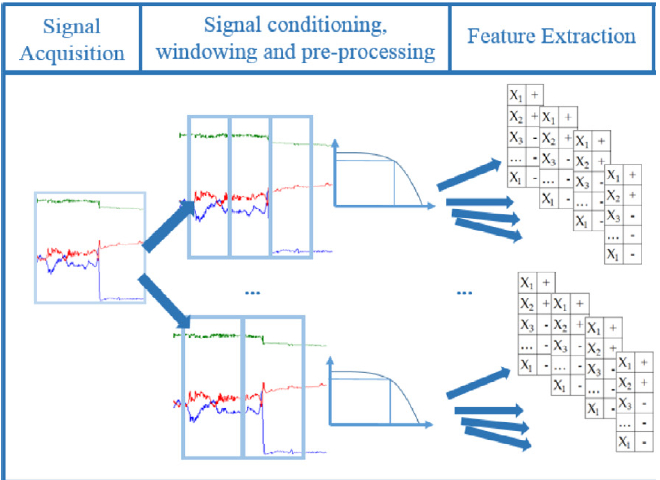
\includegraphics[scale=0.6]{images/flusso_feature.png}
	\caption{Schema generale di calcolo delle feature statistiche}
	\label{Flusso Feature}
\end{figure}

\section{Feature Dinamiche}


\section{Linear Discriminant Analysis}
